\section{Appendix}
\subsection{Plots for Quark Matter 2014 approval}
\begin{figure}[hbtp]
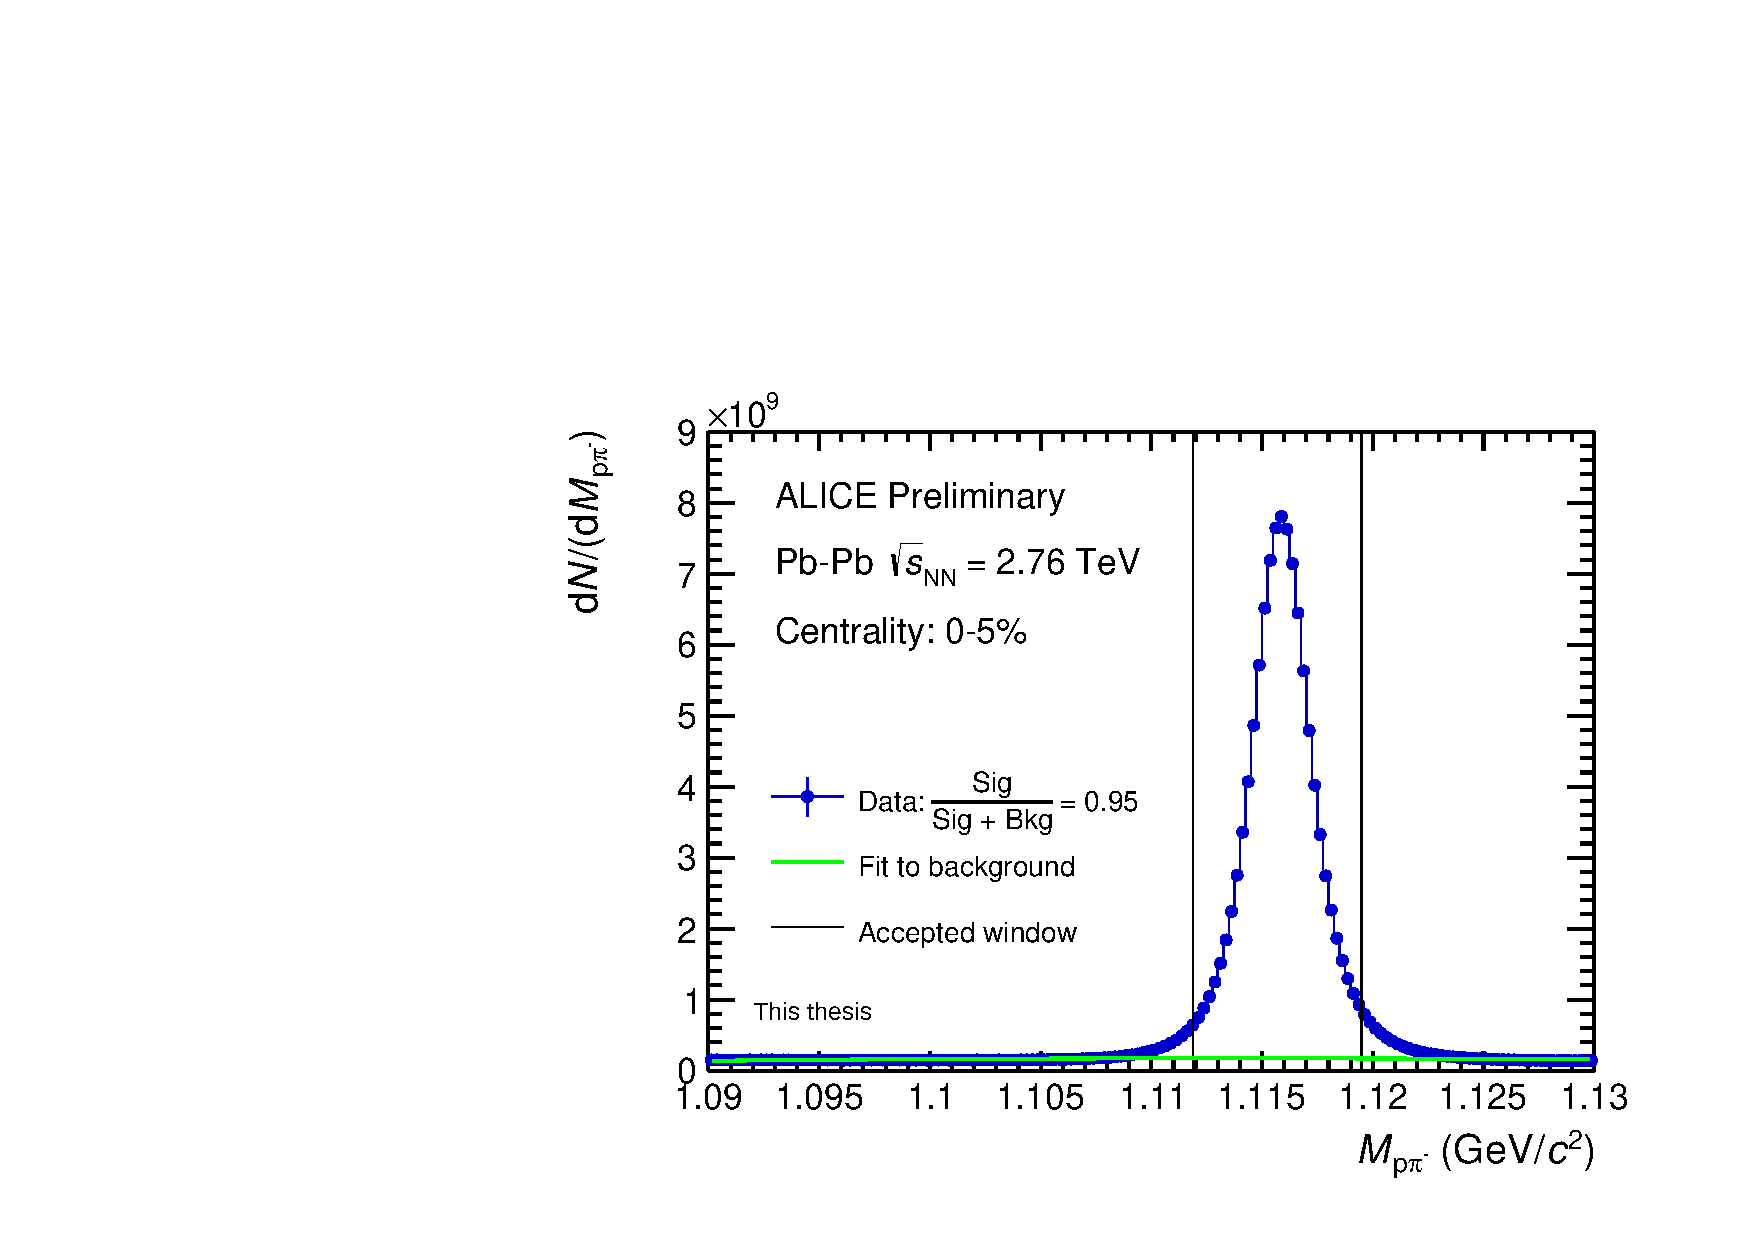
\includegraphics[width=36pc]{Figures/2014-05-11-LamMinv-CommentCorrections.pdf}
\caption[$\Lambda$ invariant mass distribution]{Invariant mass distribution for reconstructed $\Lambda$ using the optimal analysis cuts.  
The plots show V0s reconstructed from centrality integrated LHC11h data.  
The green line shows a fourth order polynomial fit to the background, which is used to estimate the number of real and fake $\Lambda$.  
The estimated ratio of real $\Lambda$ to all reconstructed $\Lambda$ in the signal region ($ \lvert m_{\mathrm{inv}} - m_{\mathrm{PDG}}\rvert < 3.8$ MeV/$\rm c^2$) is approximately 0.95.}
\label{fig:AppendixLamInvMass}
\end{figure}

\begin{figure}[hbtp]
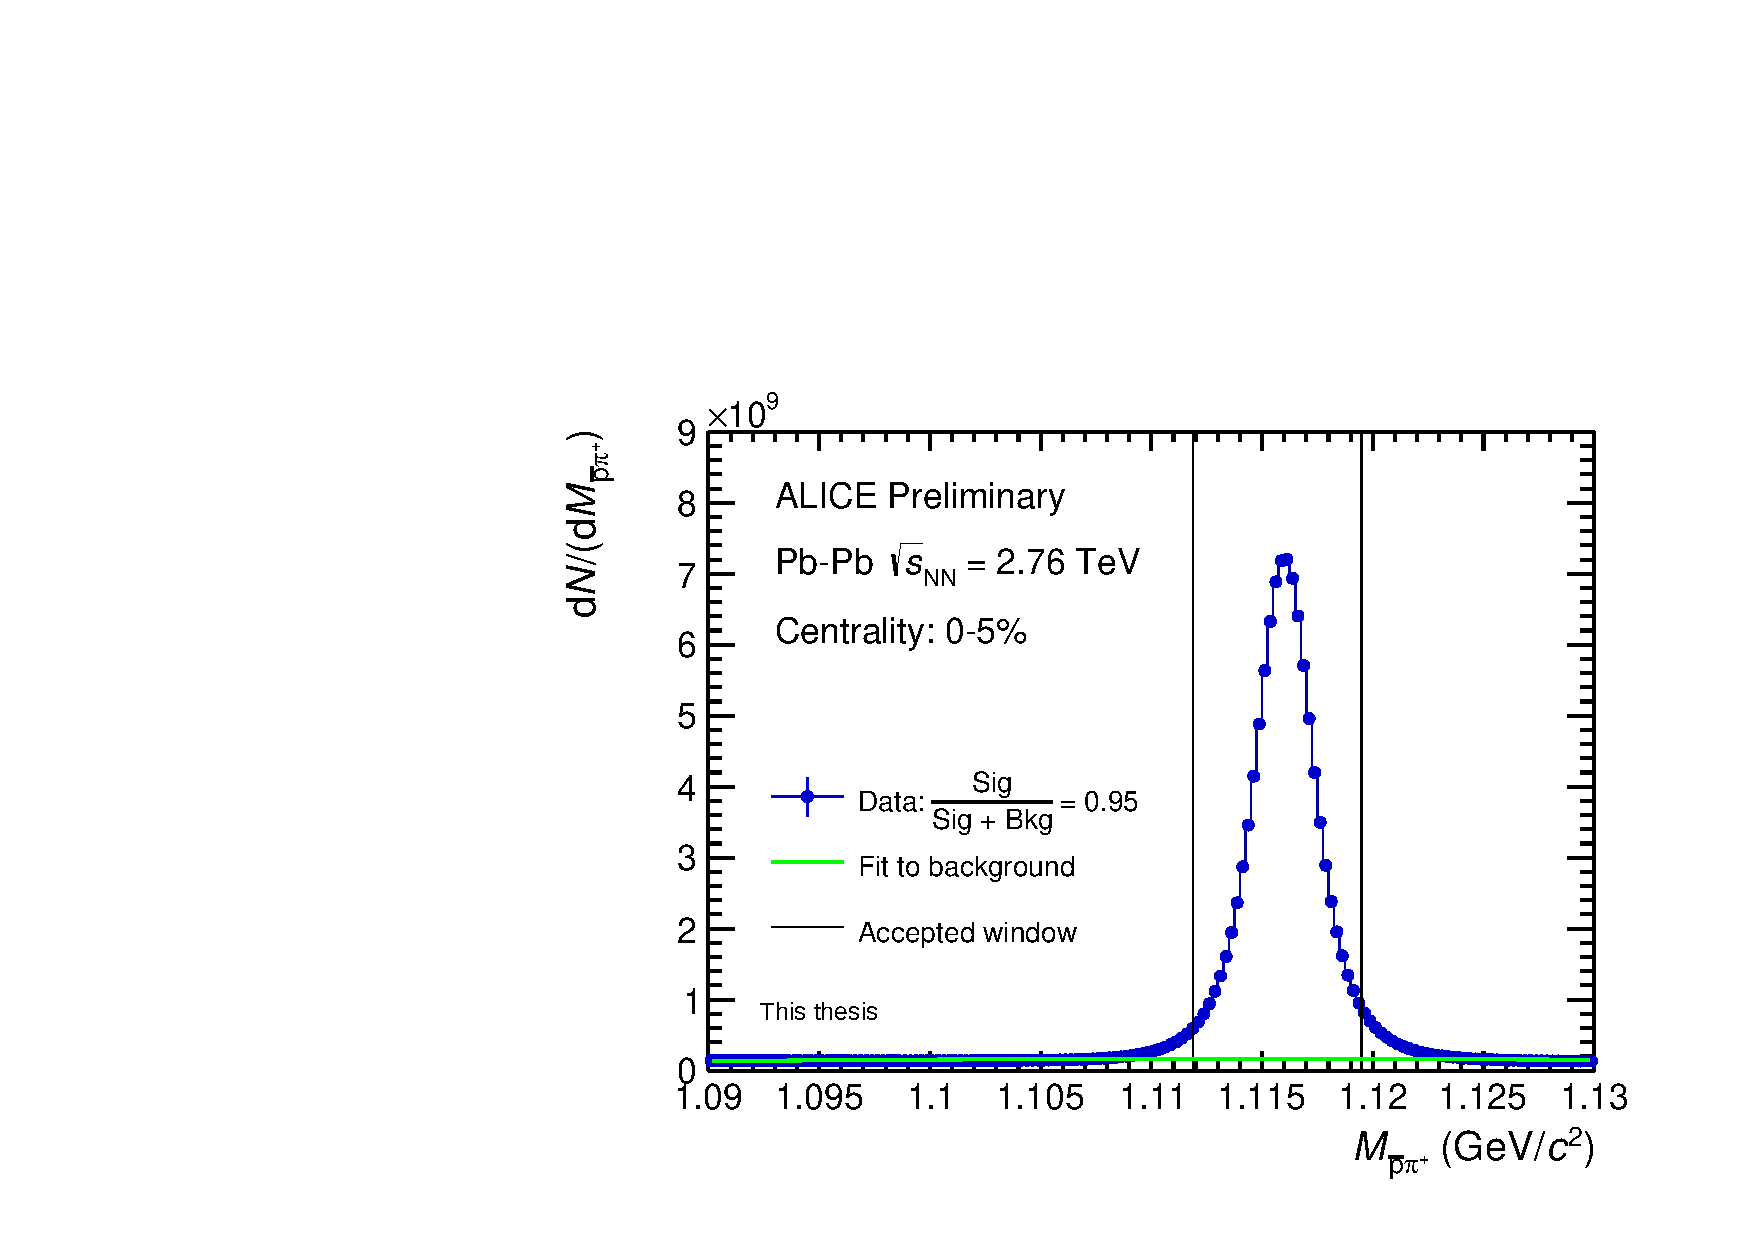
\includegraphics[width=36pc]{Figures/2014-05-11-ALamMinv-CommentCorrections.pdf}
\caption[$\bar{\Lambda}$ invariant mass distributions]{Invariant mass distribution for reconstructed $\bar{\Lambda}$ using the optimal analysis cuts.  
The plots show V0s reconstructed from centrality integrated LHC11h data.  
The green line shows a fourth order polynomial fit to the background, which is used to estimate the number of real and fake $\bar{\Lambda}$.  
The estimated ratio of real $\bar{\Lambda}$ to all reconstructed $\bar{\Lambda}$ in the signal region ($ \lvert m_{\mathrm{inv}} - m_{\mathrm{PDG}}\rvert < 3.8$ MeV/$\rm c^2$) is approximately 0.95.}
\label{fig:AppendixALamInvMass}
\end{figure}

\begin{figure}[hbtp]
\includegraphics[width=36pc]{Figures/2014-05-11-CfLLAA-010-CommentCorrections.pdf}
\caption[$\Lambda\Lambda + \bar{\Lambda}\bar{\Lambda}$ correlation function for the 0-10\% centrality range]{$\Lambda\Lambda + \bar{\Lambda}\bar{\Lambda}$ correlation function for the 0-10\% centrality range with statistical and systematic errors.  
A dip at low $k^*$ is seen which is expected from quantum interference.}
\label{fig:AppendixCFLamLamALamALam010}
\end{figure}
\begin{figure}[hbtp]
\includegraphics[width=36pc]{Figures/2014-05-11-CfLLAA-1030-CommentCorrections.pdf}
\caption[$\Lambda\Lambda + \bar{\Lambda}\bar{\Lambda}$ correlation function for the 10-30\% centrality range]{$\Lambda\Lambda + \bar{\Lambda}\bar{\Lambda}$ correlation function for the 10-30\% centrality range with statistical and systematic errors.  
A dip at low $k^*$ is seen which is expected from quantum interference.}
\label{fig:AppendixCFLamLamALamALam1030}
\end{figure}
\begin{figure}[hbtp]
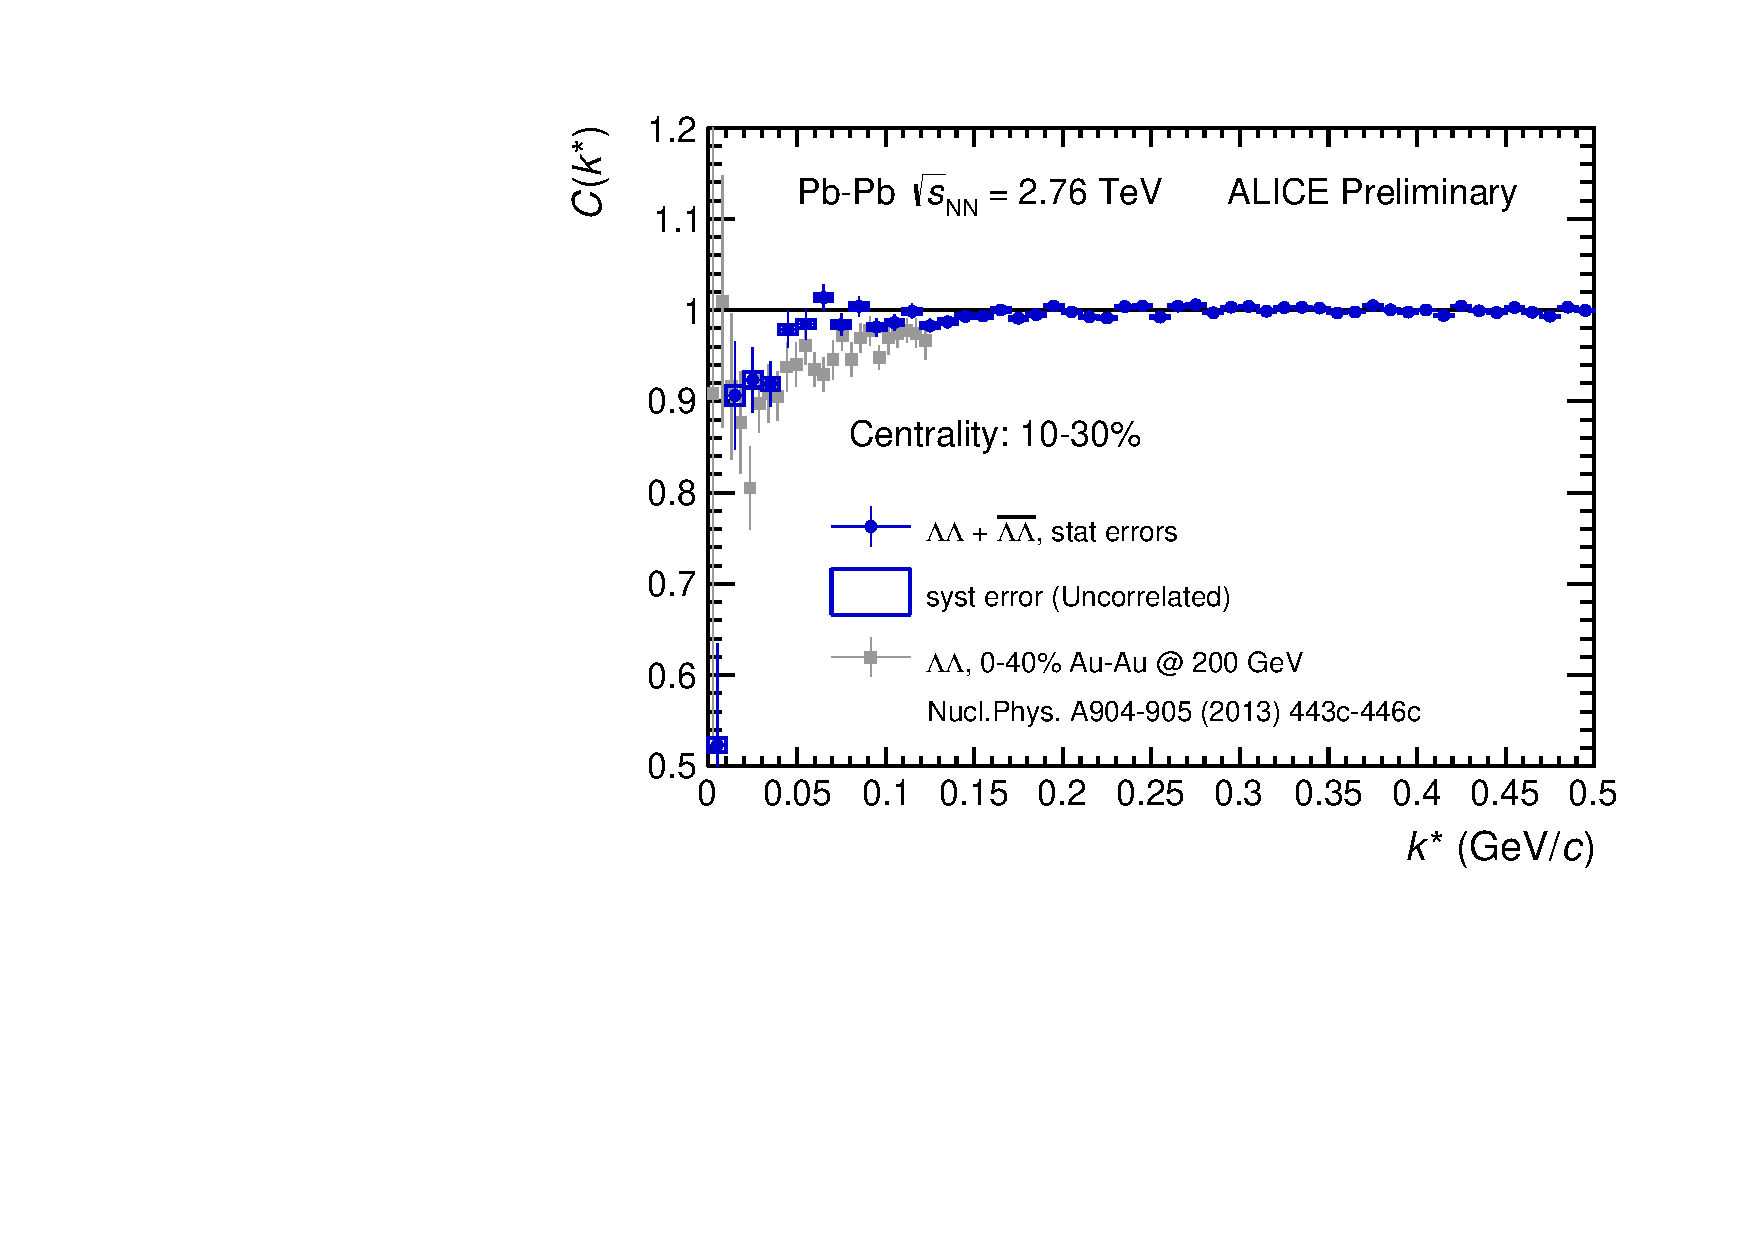
\includegraphics[width=36pc]{Figures/2014-05-11-CfLLAA-1030-CommentCorrections-WithSTAR.pdf}
\caption[$\Lambda\Lambda + \bar{\Lambda}\bar{\Lambda}$ correlation function for the 10-30\% centrality range]{$\Lambda\Lambda + \bar{\Lambda}\bar{\Lambda}$ correlation function for the 10-30\% centrality range with statistical and systematic errors.  
A dip at low $k^*$ is seen which is expected from quantum interference.  
Preliminary STAR data for $\Lambda\Lambda$ is shown for comparison.}
\label{fig:AppendixCFLamLamALamALam1030STAR}
\end{figure}
\begin{figure}[hbtp]
\includegraphics[width=36pc]{Figures/2014-05-11-CfLLAA-3050-CommentCorrections.pdf}
\caption[$\Lambda\Lambda + \bar{\Lambda}\bar{\Lambda}$ correlation function for the 30-50\% centrality range]{$\Lambda\Lambda + \bar{\Lambda}\bar{\Lambda}$ correlation function for the 30-50\% centrality range with statistical and systematic errors.  
A hint of a dip at low $k^*$ may be seen, which would be expected from quantum interference.}
\label{fig:AppendixCFLamLamALamALam3050}
\end{figure}

%\subsection{Plots currently approved}



